PMTs are used in the TRITIUM experiment for two main objectives. On the one hand, to determine the amount of incident photons that reach the PMT photocathode and, on the other hand, to measure the energy spectrum of tritium events in the laboratory prototypes.

To determine the amount of photons reaching the photocathode, the PMT should work without gain which is a source of uncertainty. For this, the bias circuit shown in Figure \ref{fig:ElectronicSchemeBasePMTNoGain} was employed. As electrons are not multiplied, the output current of the photosensor is very small (currents in the nanoampere range). This output current was read out by a Keithley 6487 Picoammeter/Voltage Source \cite{DataSheetKeithley6487}. 

The energy of the events was measured using PMTs powered with the voltage divider shown in Figure \ref{fig:VoltageDividerCircuit}. A scheme of the electronics is shown in Figure \ref{fig:ElectronicConfiguraitonsPMT}.
\begin{figure}
\centering
    \begin{subfigure}[b]{1.0\textwidth}
    \centering
    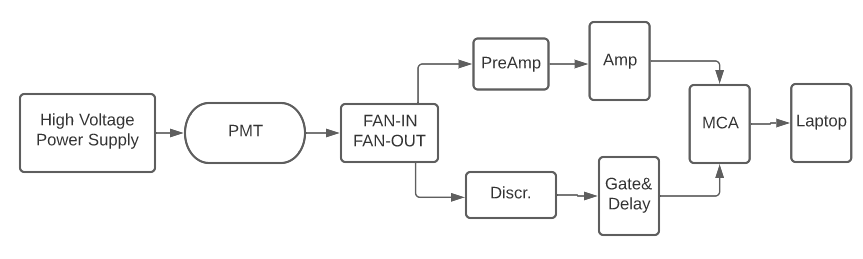
\includegraphics[width=\textwidth]{3DesignPrinciples/32Tritium_detector/Electronical_Scheme_1_PMT.png}  
    \caption{\label{subfig:ElectronicConfiguraiton1PMT}}
    \end{subfigure}
    \hfill
    \begin{subfigure}[b]{1.0\textwidth}
    \centering
    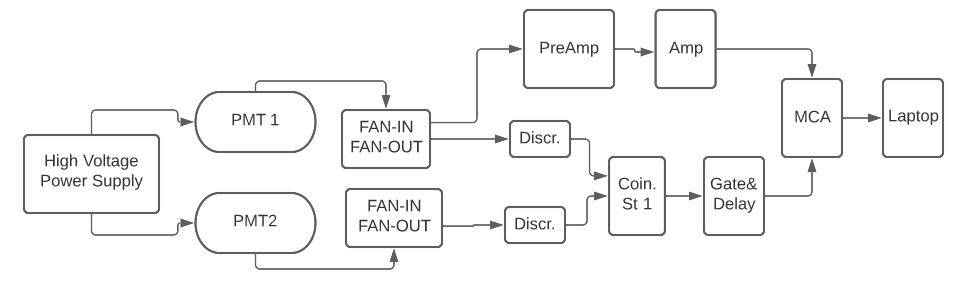
\includegraphics[width=\textwidth]{3DesignPrinciples/32Tritium_detector/Electronical_Scheme_2_PMTs.png}  
    \caption{\label{subfig:ElectronicConfiguraiton2PMT}}
    \end{subfigure}
    \hfill
    \begin{subfigure}[b]{1.0\textwidth}
    \centering
    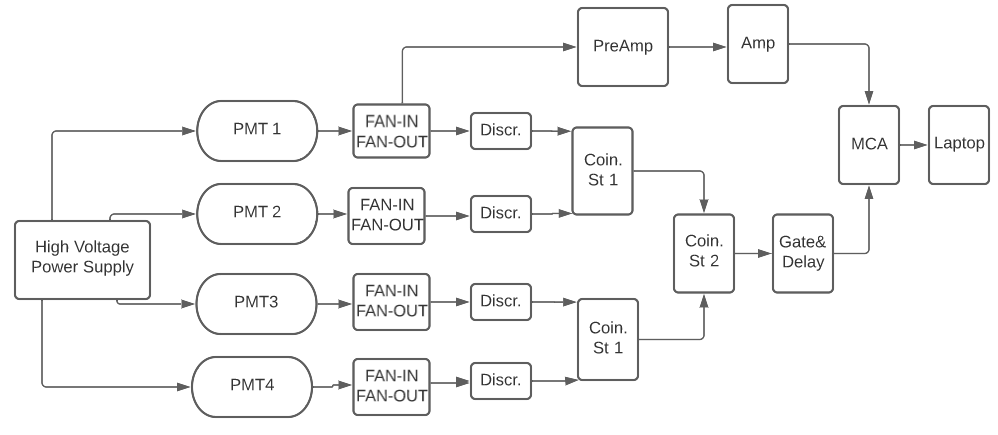
\includegraphics[width=\textwidth]{3DesignPrinciples/32Tritium_detector/Electronical_Scheme_4_PMTs.png}  
    \caption{\label{subfig:ElectronicConfiguraiton4PMT}}
    \end{subfigure}
 \caption{Electronic schemes employed for measuring with a) one PMT, b) two PMTs in coincidence and c) four PMTs in coincidence.}
 \label{fig:ElectronicConfiguraitonsPMT}
\end{figure}
The PMTs were powered by a TC 952 High Voltage Supply from Tennelec \cite{DataSheetHVSupplyTennelec} and a HV Power Supply N 1130-4 from Wenzel Elektronik \cite{DataSheetHVSupplyWenzel}. The PMT output signals were split by an analog FAN IN-OUT model 740 from Phillips Scientific \cite{DataSheetFANINOUT} to feed the amplification and time coincidence lines. The amplification line consists of a preamplifier, model 9326 FAST PREAMP from ORTEC \cite{DataSheetPreAmp}, which gives an output signal with a heigth proportional to the charge of the input pulse and of an amplifier, model 575A or 671 from ORTEC \cite{DataSheet575Amp, DataSheet671Amp}, which produces a Gaussian shaped output signal. An example of the 575A amplifier output signal is shown in Figure \ref{fig:InputSignalsMCA}, green color. 

The time coincidence line consists of the following branches:

\begin{enumerate}

\item{}  A constant fraction discriminator, either module CF8000 from ORTEC \cite{DataSheetDiscriminator} or model 84 from CAEN \cite{DataSheetDiscriminatorCAEN}.

\item{} In the case of two or four PMTs, a coincidence module either 465 from LeCroy \cite{DataSheetCoincidenceLeCroy} or Coincidence Type N6234 from CERN-NP \cite{DataSheetCoincidenceCERN}, used to generate an output signal of $20~\ns$ width when both inputs are in coincidence. 

\item{} In the case of four PMTs, an additional coincidence stage is employed. In Figure \ref{fig:DifferentCoincidences}, time coincidences of 4 PMTs are shown. Case d) shows coincident events.

%In Figure \ref{fig:DifferentCoincidences}, time coincidences of two detectors (4 PMTs) are shown. The four logic signals are displayed, two of them from each detector. The possible cases are:

%\begin{enumerate}
%\item{} Only one PMT (channel two) detected an event as shown in Figure \ref{subfig:signalInOnePMT}. It means that the event is likely not produecd in the detector. In this case, no output signal is generated.

%\item{} Two PMT signals are generated but the other detector gives no signal as shown in Figures \ref{subfig:signalInTwoPMTOneDetector} and \ref{subfig:signalInTwoPMTOtherDetector} . This event is discarded.

%\item{} The four signals are generated as shown in Figure \ref{subfig:signalInAllPMTsBothDetector}  and, consequently, the output signal is generated and the event is recorded.

\begin{figure}
\centering
    \begin{subfigure}[b]{0.45\textwidth}
    \centering
    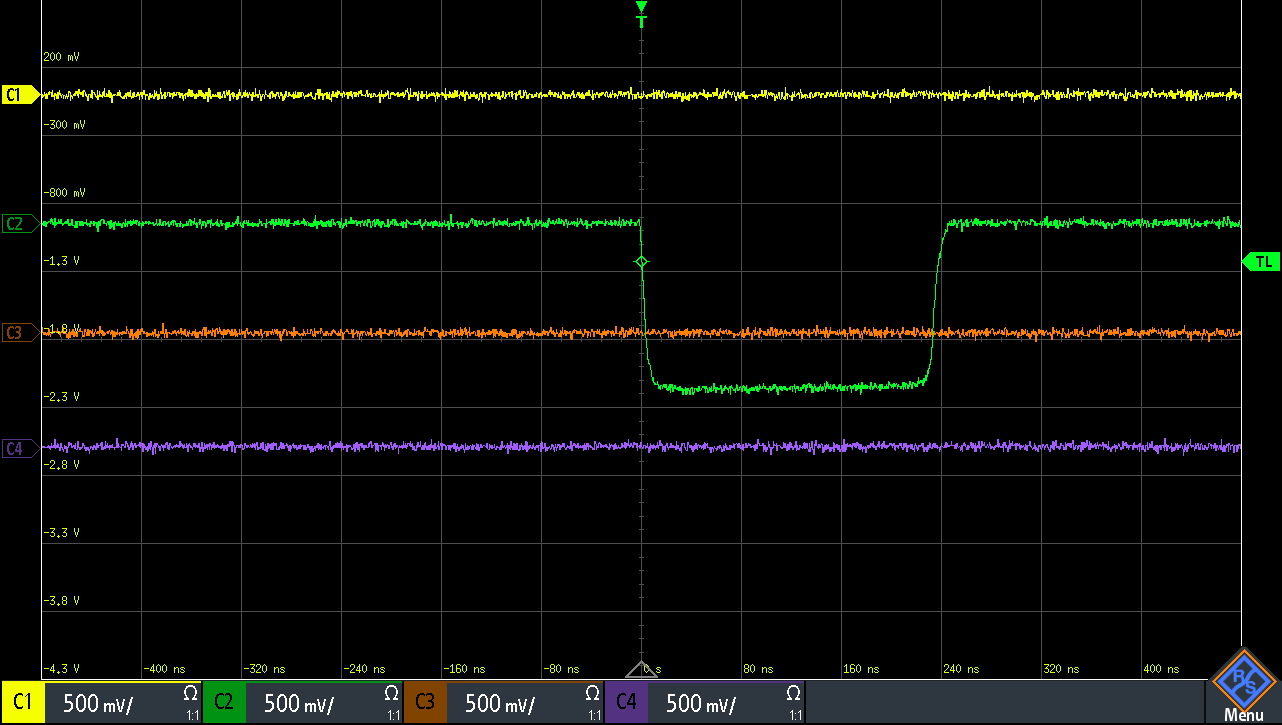
\includegraphics[width=\textwidth]{3DesignPrinciples/32Tritium_detector/1_coincidences.png}  
    \caption{\label{subfig:signalInOnePMT}}
    \end{subfigure}
    \hfill
    \begin{subfigure}[b]{0.45\textwidth}
    \centering
    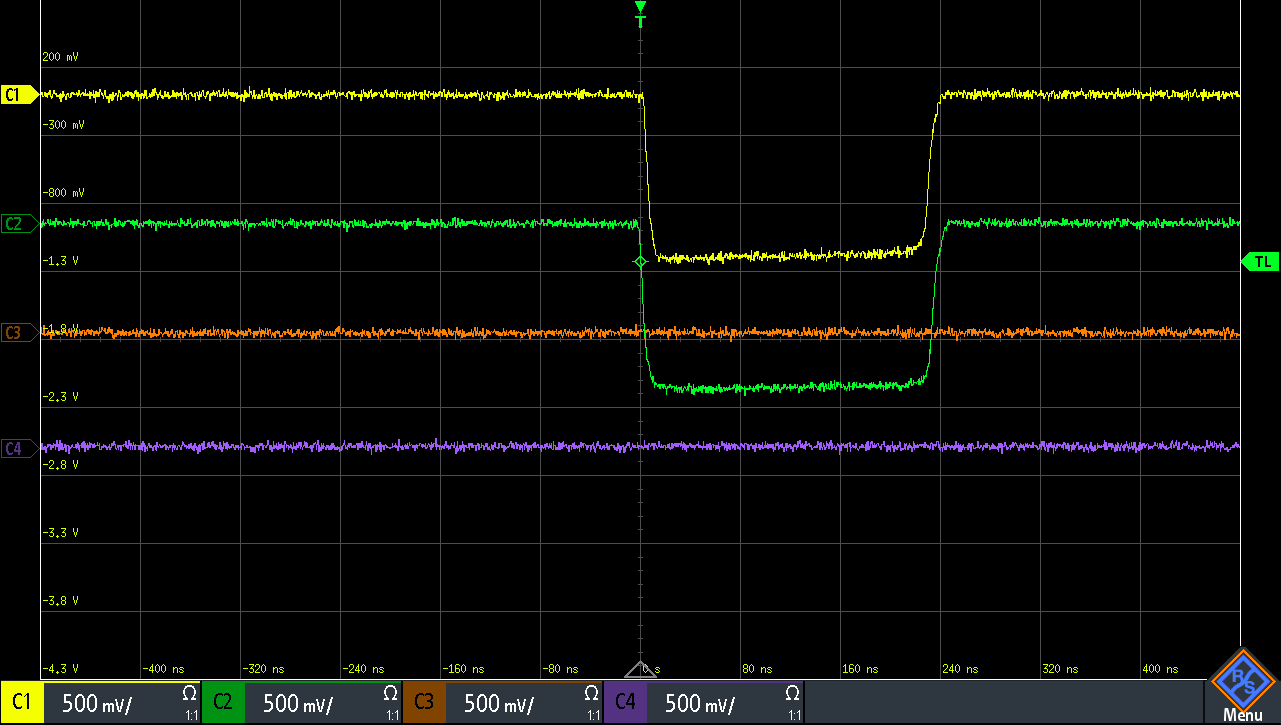
\includegraphics[width=\textwidth]{3DesignPrinciples/32Tritium_detector/2_coincidences_1.png}  
    \caption{\label{subfig:signalInTwoPMTOneDetector}}
    \end{subfigure}
    \hfill
    \begin{subfigure}[b]{0.45\textwidth}
    \centering
    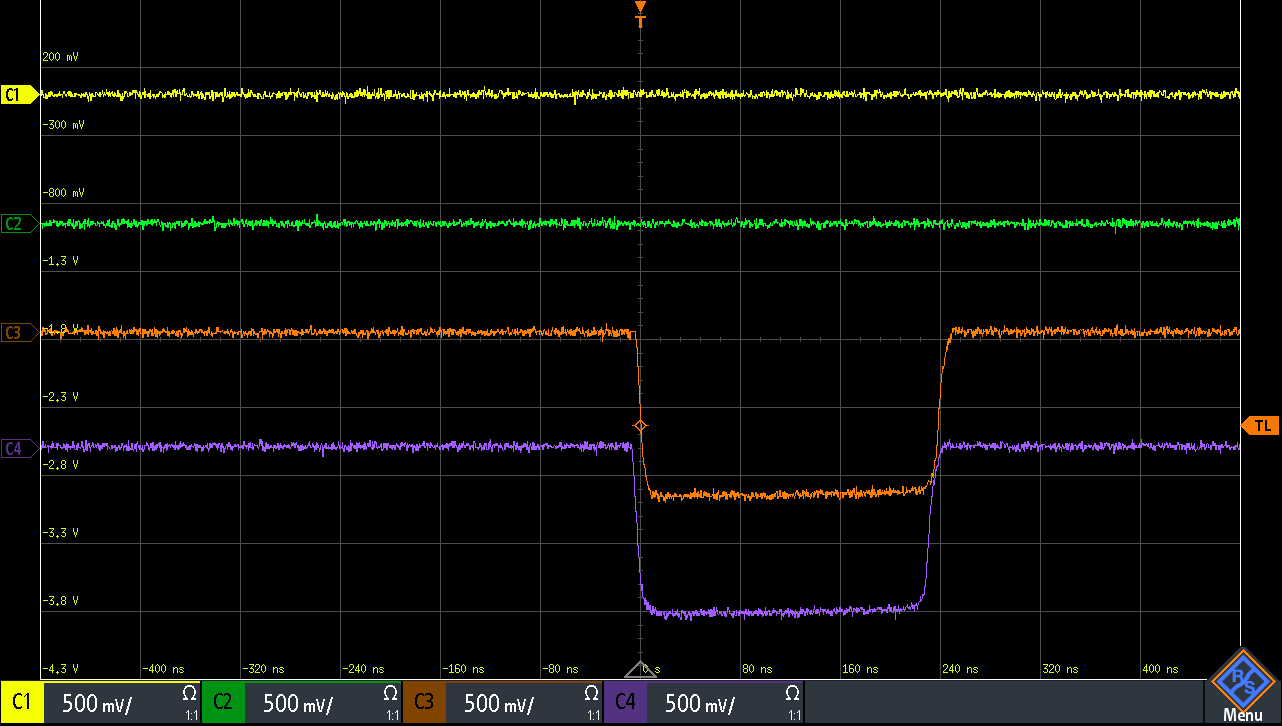
\includegraphics[width=\textwidth]{3DesignPrinciples/32Tritium_detector/2_coincidences_2.png}  
    \caption{\label{subfig:signalInTwoPMTOtherDetector}}
    \end{subfigure}
    \hfill
    \begin{subfigure}[b]{0.45\textwidth}
    \centering
    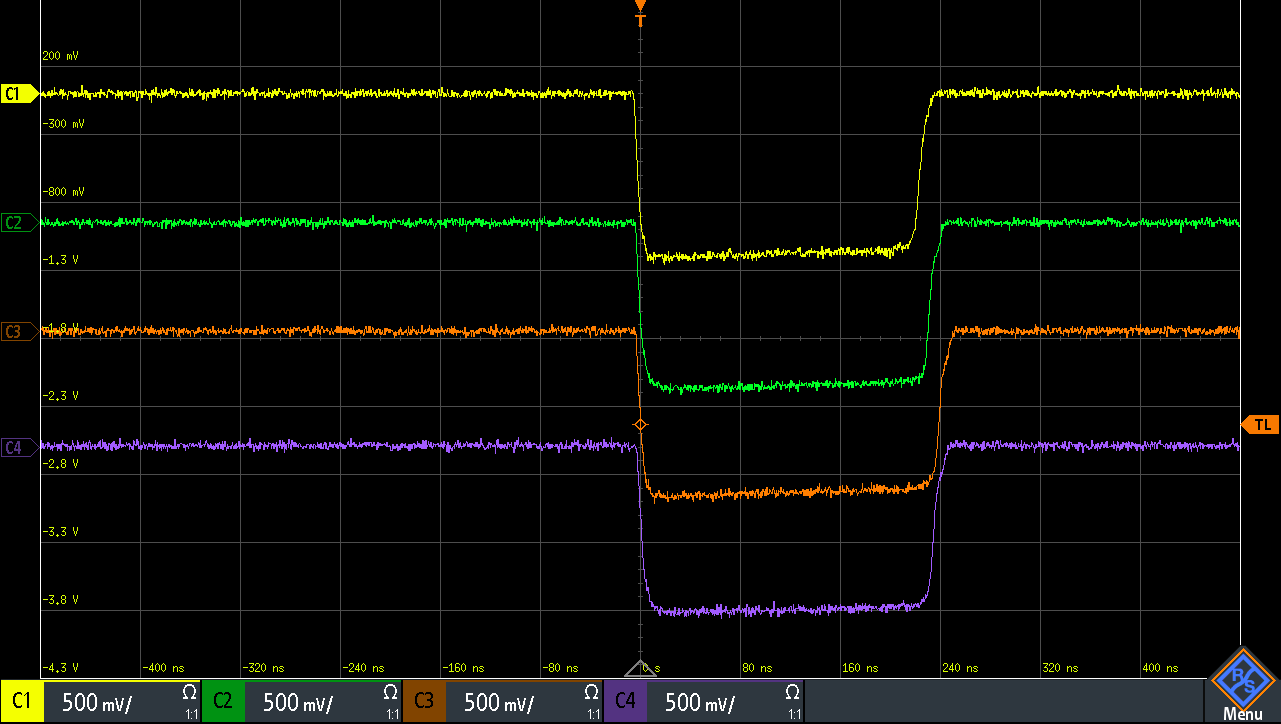
\includegraphics[width=\textwidth]{3DesignPrinciples/32Tritium_detector/4_coincidences.png}  
    \caption{\label{subfig:signalInAllPMTsBothDetector}}
    \end{subfigure}
 \caption{Different possibilities for time coincidence of four PMTs. Case d) shows coincident events.}
 \label{fig:DifferentCoincidences}
\end{figure}

\item{} A Gate and Delay Generator, model 416A from ORTEC \cite{DataSheetGateAndDelay}, which produces a positive logic signal of $8~\volt$ height and $2~\mu\second$ width. This module delays the time windows until they overlap with the energy signal as shown in Figure \ref{fig:InputSignalsMCA}.

\end{enumerate}

The energy signal and the coincidence signal, shown in Figure \ref{fig:InputSignalsMCA}, are recorded by a MCA model 8000D from AMPTEK \cite{DataSheetMCA}.

\begin{figure}[htbp]
\centering
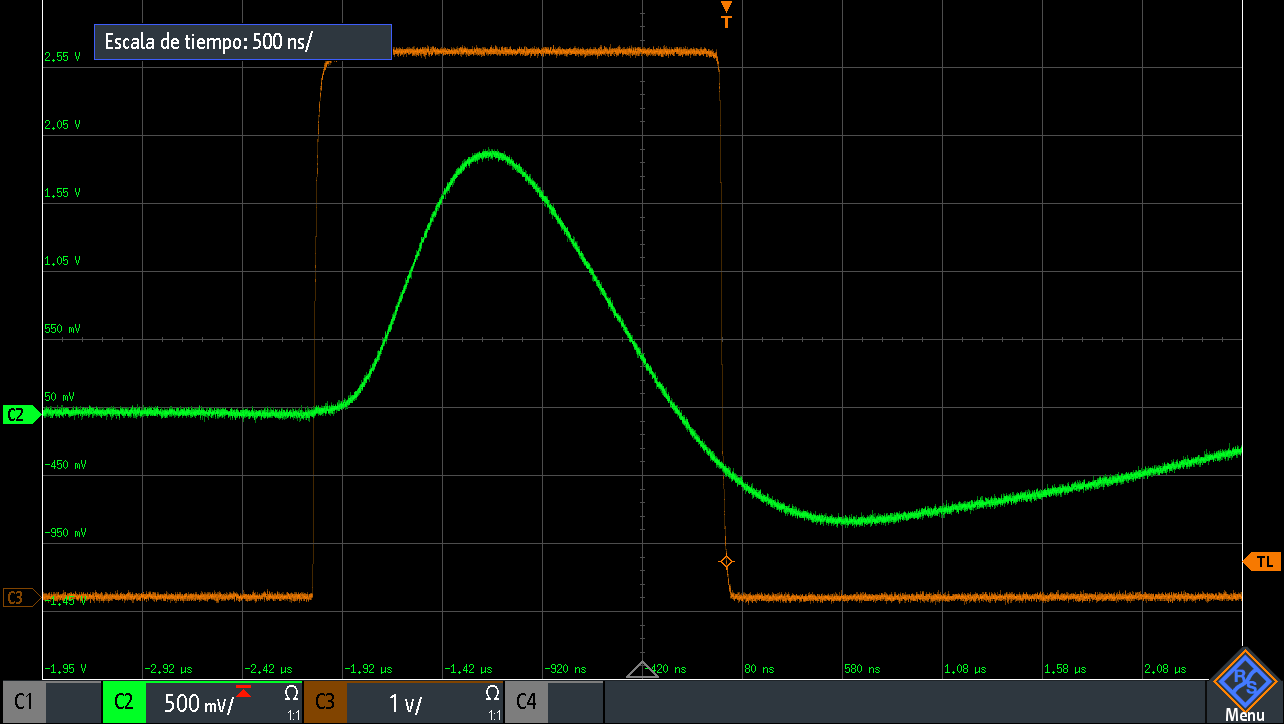
\includegraphics[scale=0.3]{3DesignPrinciples/32Tritium_detector/Input_MCA.png}
\caption{Amplified signal and logic gate (input signals of the MCA).\label{fig:InputSignalsMCA}}
\end{figure}